    \subsection*{Evaluating our Learning Algorithm}
    
        So, while we can evaluate each \textbf{hypothesis}, it's also important to measure how our \textbf{learning algorithm} is performing.
        
        How do we measure it? Well, the job of our \textbf{learning algorithm} is to \textbf{pick good hypotheses}.\\
        
        \begin{concept}
            We can \vocab{evaluate} the performance of a \vocab{learning algorithm} using \purp{testing loss}: a good learning algorithm will create \gren{hypotheses} with \purp{low testing loss}.
        \end{concept}
        
        You could think of this as measuring the \textbf{skill} of a \textbf{teacher} (the learning algorithm) by the \textbf{success} of their \textbf{student} (the hypothesis) on a \textbf{test} (testing loss).
        
    \subsection*{Validation: Evaluating with lots of data}
    
        When we were creating hypotheses, \textbf{randomness} caused some problems: you might not get \textbf{training data} that matched the \textbf{testing data} very well.
        
        The \textbf{same} can happen here, when \textbf{evaluating} your \textbf{algorithm}: maybe your model happened to create a bad (or unusually good!) hypothesis because of \textbf{luck}.
        
        The easy solution to \textbf{randomness} is to add \textbf{more data}: we get more \textbf{consistency} that way.
        
        So, we \textbf{repeatedly} get new training data and test data. For each, we \textbf{train} a different hypothesis. We can \textbf{average} their performance out, and use that to \textbf{estimate} the quality of our algorithm.\\
        
        \begin{definition}
            \vocab{Validation} is a way to \vocab{evaluate a learning algorithm} using \vocab{large amounts of data}.
            
            We do this by \gren{running} our algorithm \purp{many times} with new data, and \gren{averaging} the testing error of all the hypotheses.
            
            This process is often requires having \purp{lots of data} to train with, but is a \textbf{provably} good approach.
        \end{definition}
        
    \subsection*{Our Problem: When data is less available}
        
        As mentioned, this takes up \textbf{lots of data}. What if we can't get as much: it's \textbf{expensive}, or not even possible? In this case, we have some \textbf{finite} data, $\data_n$. We \textbf{can't get more}.
        
        We solved the \textbf{randomness} problem by using \textbf{more} training and testing \textbf{data}. So, we need some way to \textbf{get} more \textbf{distinct} hypotheses.
        
        One set of data gives us one \textbf{hypothesis}. But, what if, rather than using \textbf{completely} new data, we used \textbf{slightly different} data each time?
        
        First, need to break $\data_n$ into a chunk for training, and a chunk for testing.
        
        \begin{figure}[H]
        \centering
            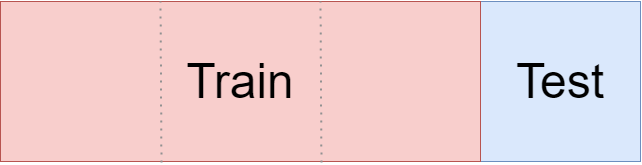
\includegraphics[width=70mm,scale=0.5]{images/regression_images/training_and_test_data.png}
        \end{figure}
        
        How do we get more hypotheses from this dataset?
        
    \subsection*{Cross-Validation}
    
        We mentioned that we just want \textbf{different} hypotheses. Our hypotheses depend on our \textbf{training data}. So we want to \textbf{change} our training data.
        
        We can't \textbf{add} data to it, because then we \textbf{lose} testing data. We shouldn't \textbf{remove} data, because then we're just making a hypothesis that's \textbf{less well-informed}.
        
        Instead, we'll \textbf{swap} some of the training data for testing data.
        
        \begin{figure}[H]
        \centering
            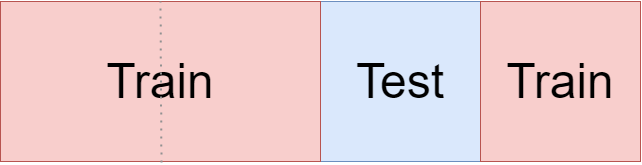
\includegraphics[width=70mm,scale=0.5]{images/regression_images/training_and_test_data_2.png}
        \end{figure}
        
        This will create a new hypothesis, and the data is partially different! In fact, we can do this for each of our chunks:
        
        \begin{figure}[H]
        \centering
            \begin{subfigure}
                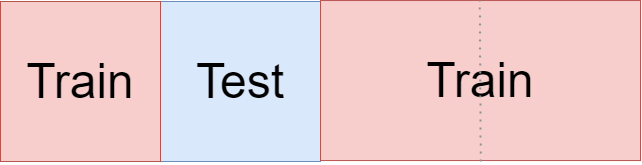
\includegraphics[width=70mm,scale=0.5]{images/regression_images/training_and_test_data_3.png}
            \end{subfigure}
            \\
            \begin{subfigure}
                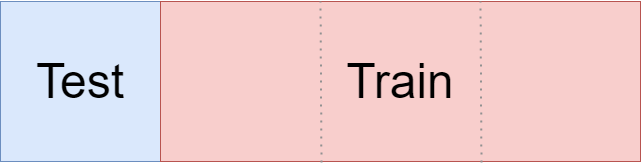
\includegraphics[width=70mm,scale=0.5]{images/regression_images/training_and_test_data_4.png}
            \end{subfigure}
            
        \end{figure}
        
        We now have \textbf{four different hypotheses} for the price of one!\\
        
        \begin{definition}
            \vocab{Cross-validation} is a way to \vocab{evaluate a learning algorithm} using \vocab{limited data}.
            
            We do this by \purp{breaking} our data it into \gren{chunks} to create \purp{multiple hypotheses} from one dataset.
            
            For each \gren{chunk}, we train one dataset on all the data \textbf{not in that chunk}. We get our \purp{test error} using the chunk \textbf{we left out}.
            
            For $k$ chunks, we end up with $k$ hypotheses. By \gren{averaging} out their performance, we can \purp{approximate} the quality of our algorithm.
        \end{definition}
        
        This approach is much \textbf{less expensive}, and very common in machine learning! But, some of the theoretical \textbf{benefits} of validation are not \textbf{proven} to be true for cross-validation.\\
        
        \begin{clarification}
            Note that the goal of validation and cross-validation is \textbf{not} to evaluate \purp{one hypothesis}.
            
            Instead, it is instead meant to evaluate a \purp{learning algorithm}. This is why we have to create \purp{many} hypotheses: we want to see that our algorithm is \gren{generally} good!
        \end{clarification}